% Overizcht feest:
% Datum \$DATUMFEEST
% Aantal gasten \$GROEPGROTE
% Waarvan kinderen \$KINDEREN
% Betreft: \$BETREFT
% Begintijd: \$BEGINTIJD
% \$STARTPLANNING

\documentclass{letter}
\usepackage[dutch]{babel}
\usepackage{fancyhdr}
\usepackage{wallpaper}
\usepackage[official]{eurosym}
\usepackage{background}
\usepackage{url}
\usepackage{enumitem}
\setlist{nosep, after=\vspace{\baselineskip}}

% weird character support (ie sate).
\usepackage[utf8]{inputenc}
\usepackage[T1]{fontenc}
\usepackage{lmodern} % load a font with all the characters


\setcounter{secnumdepth}{0}% % Turns off numbering for sections
\makeatletter
\usepackage{etoolbox}% http://ctan.org/pkg/etoolbox
\patchcmd{\@sect}% <cmd>
  {\else \protect}% <search>
  {\protect\numberline{}\else\protect}% <replace>
  {}{}% <success><failure>
\makeatother 

\graphicspath{{img/}}

\backgroundsetup{
  scale=1.2,
  color=black,
  opacity=1,
  angle=0,
  position=current page.south,
  vshift=110pt,
  hshift=50pt,
  contents={%
  \begin{minipage}{.8\textwidth}
	\center
	\large Restaurant De Huiskamer \\
	\tiny Kerkdijk 2 - 7964KB Ansen - tel 0522-471280 - KvK 04005343 -  info@dehuiskamer.com \\
	IBAN NL07 SNSB 095.65.49.721 - BTW nr: 8094.43867B01 \\
	\url{www.dehuiskamer.com} - \url{www.de2dekamer.nl} - \url{www.facebook.com/RestaurantDeHuiskamer}
  \end{minipage}\hspace{-.05\textwidth}%
  \begin{minipage}{.18\textwidth}
  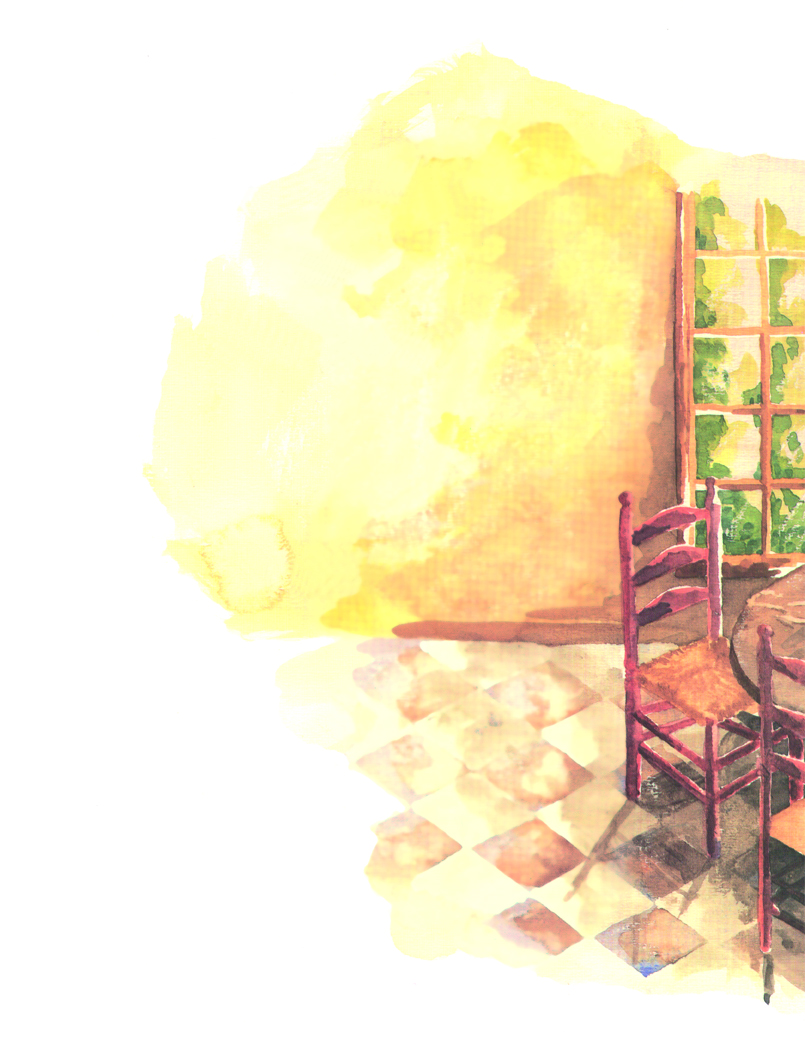
\includegraphics[width=\linewidth,height=110pt,keepaspectratio]{logo2kleur}
  \end{minipage}%
  }
}

\pagestyle{fancy}
\cfoot{}
\renewcommand\headrulewidth{0pt}
\chead{\large Restaurant De Huiskamer \\
\small Ansen $\quad$ tel $0522-471280$}
\begin{document}
\ThisURCornerWallPaper{0.25}{img/logo.jpg}

\signature{Pedro Klooster}
\address{\$NAAM \\ \$ADRESS \\ \$POSTCODE \$PLAATS}
\begin{letter}{
\textbf{Betreft: offerte}\\%
  E-mail \$EMAIL  \\
  Tel \$TEL
	}
\thispagestyle{empty}


\opening{Geachte \$AANHEF \$NAAM,}

Naar aanleiding van ons gesprek ontvangt u hierbij een vrijblijvend offerte voorstel
voor een \$BETREFT op \$DATUMFEEST \\

Uitgaande van \$GROEPGROTE gasten incusief \$KINDEREN kinderen kan dit er als volgt uit zien: \\\\
\$DRAAIBOEK

\newpage


\textbf{Kosten specificatie}
Uigaande van \$GROEPGROTE gasten inclusief \$KINDEREN kinderen.

\$PRIJSOVERZICHT

\textbf{Bijzonderheden}

\$BIJZONDERHEDEN

\$EXTRAPUNTEN

We hopen uw wensen op de juiste wijze te hebben vertaald, in afwachting op uw reactie, \\

\closing{Met gastvije groet,}
\encl{Activiteit details \\ Dieet specificaties}


\end{letter}

\newpage

\textbf{Activiteit details}

\$ACTIVITEITDETAILS

\textbf{Dieet specificaties}

\$DIEET
\end{document}
